\documentclass[12pt]{article}

\usepackage{hyperref}
\usepackage{graphicx}

\begin{document}

\title{PocketAlchemy Product Overview - v0.1.alpha}
\author{Cody J. Weaver}
\date{Dec. 31th 2023}
\maketitle

\section{v1.1.alpha Product Overview}

\indent Version 0.1.alpha is the second named version of PocketAlchemy.
This document looks to give an overview of this project as of 
Dec. 30th 2023 and provide general documentation and notes 
about PocketAlchemy.


PocketAlchemy v0.1.alpha encapsulates some major design decisions.
First I choose to use Firebase's Authentication and Firestore products.
This required setting up a Firebase project which can be found 
\href{https://console.firebase.google.com/u/0/project/pocketalchemy-c2355/overview}
{here}. Currently, PocketAlchemy can be used in the following way:


\begin{itemize}
    \item User can log in as a guest to PocketAlchemy. Logging in
    as a guest will allow a user's data to persist until the user
    either clears internal storage or uninstalls the app which will result in logging in as 
    different user anonymously the next time they 
    log in on that given device, in effect, resetting their data.
    See \S\@ 2.1 for a look at the login screen.

    \item After logging in, user is presented with a list of their recipes.
    The recipe list screen offers a button that will launch the creation of 
    a new recipe. Clicking on an individual recipe on the list will launch 
    a screen that allows the user to edit the recipe. See \S\S\@ 2.2-2.5 for 
    screenshots of the recipe list view, and the edit recipe view.
    
\end{itemize}




\section{Screenshots}
\subsection{Login Screen}

\begin{center}

\includegraphics[scale=0.175]{../res/img/LoginScreenDark.png}

\includegraphics[scale=0.175]{../res/img/LoginScreenLight.png}
\end{center}

\subsection{Recipe List (Empty)}

\begin{center}
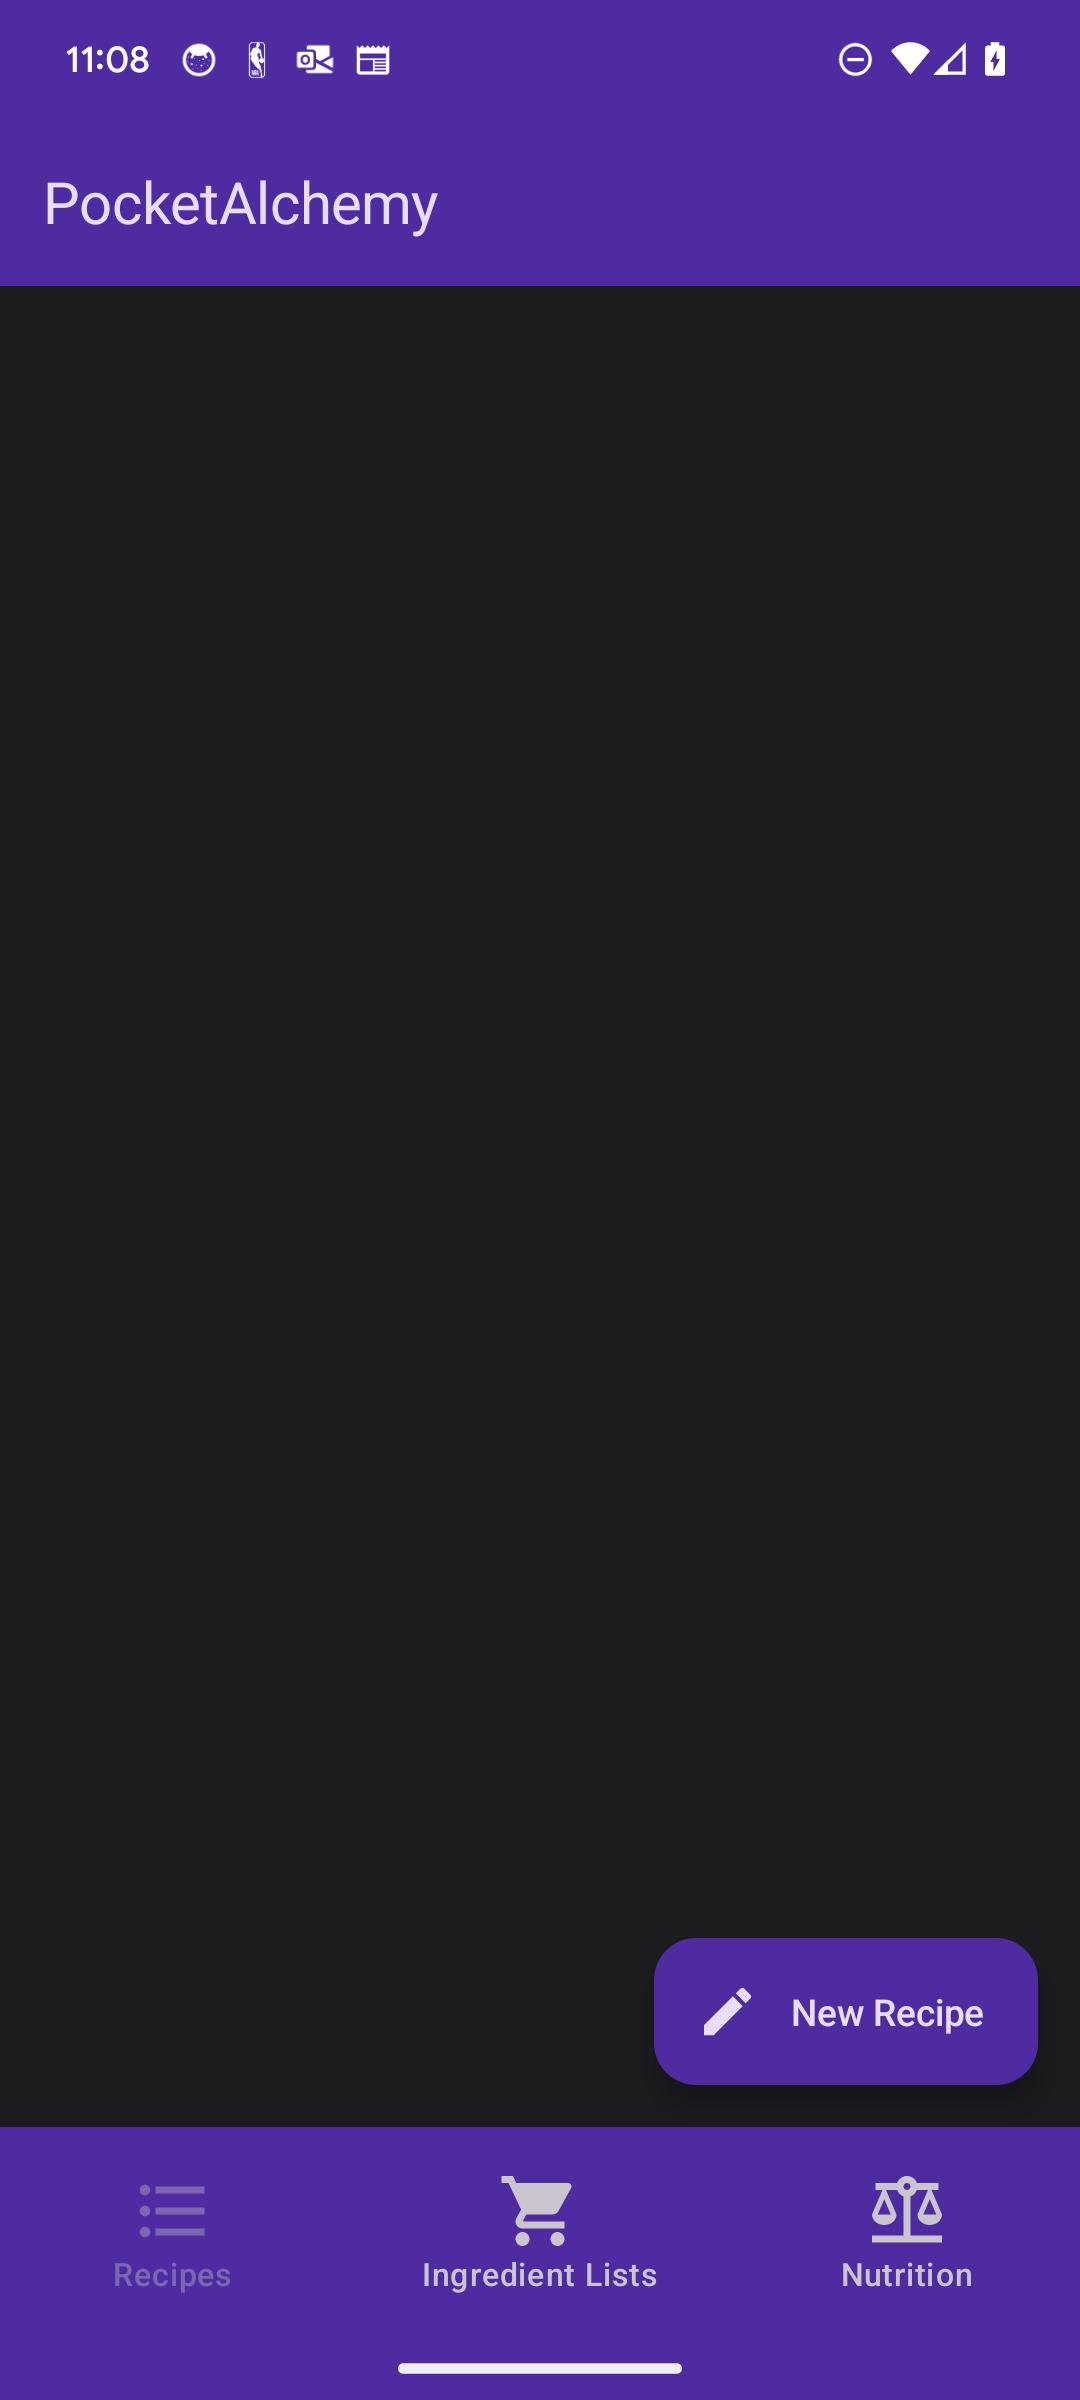
\includegraphics[scale=0.175]{../res/img/EmptyListDark.png}
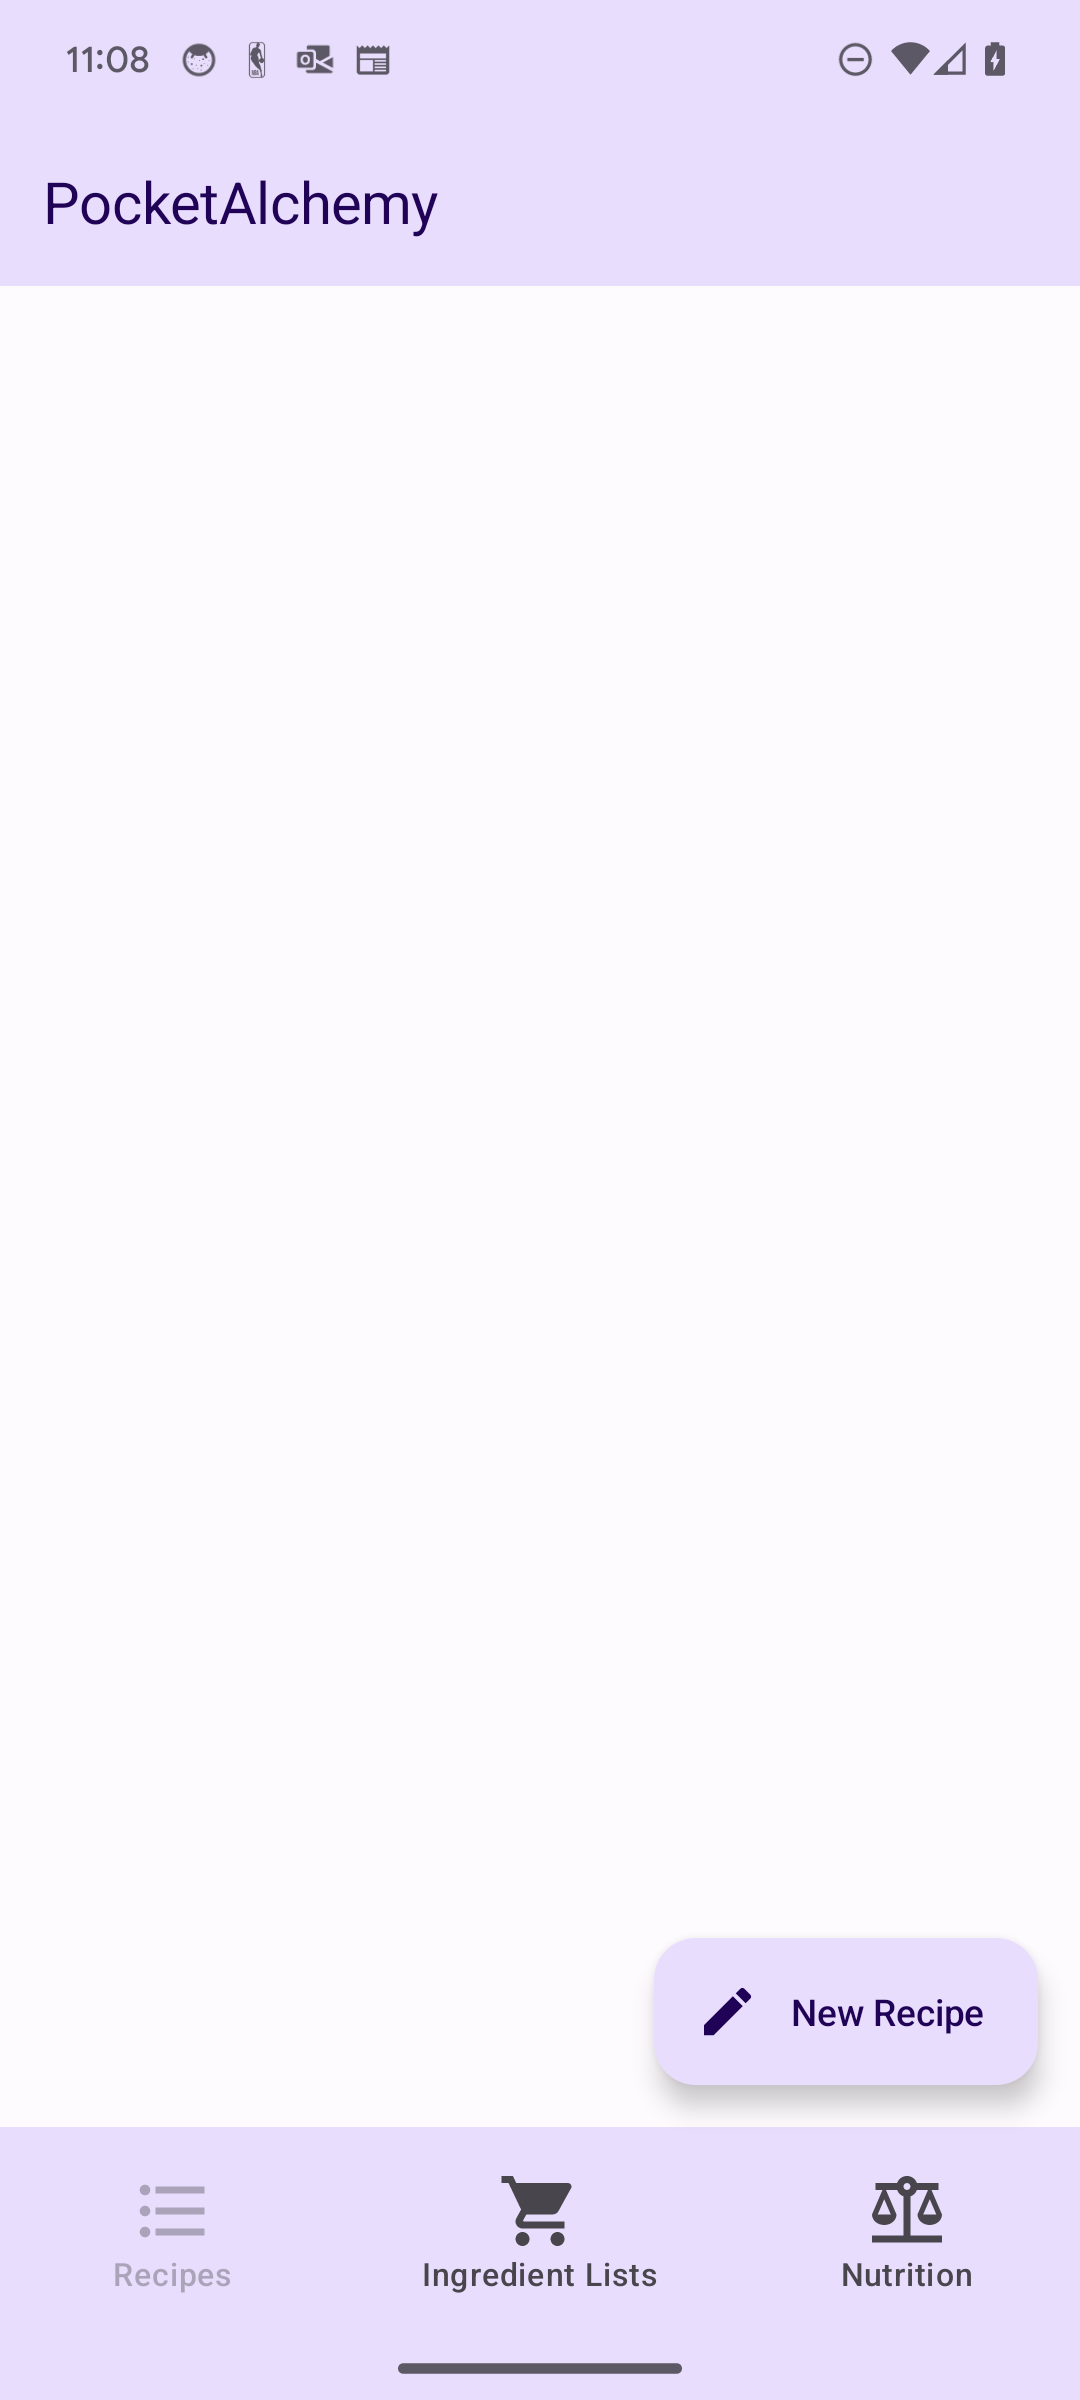
\includegraphics[scale=0.175]{../res/img/EmptyListLight.png}
\end{center}

\subsection{Recipe List}

\begin{center}
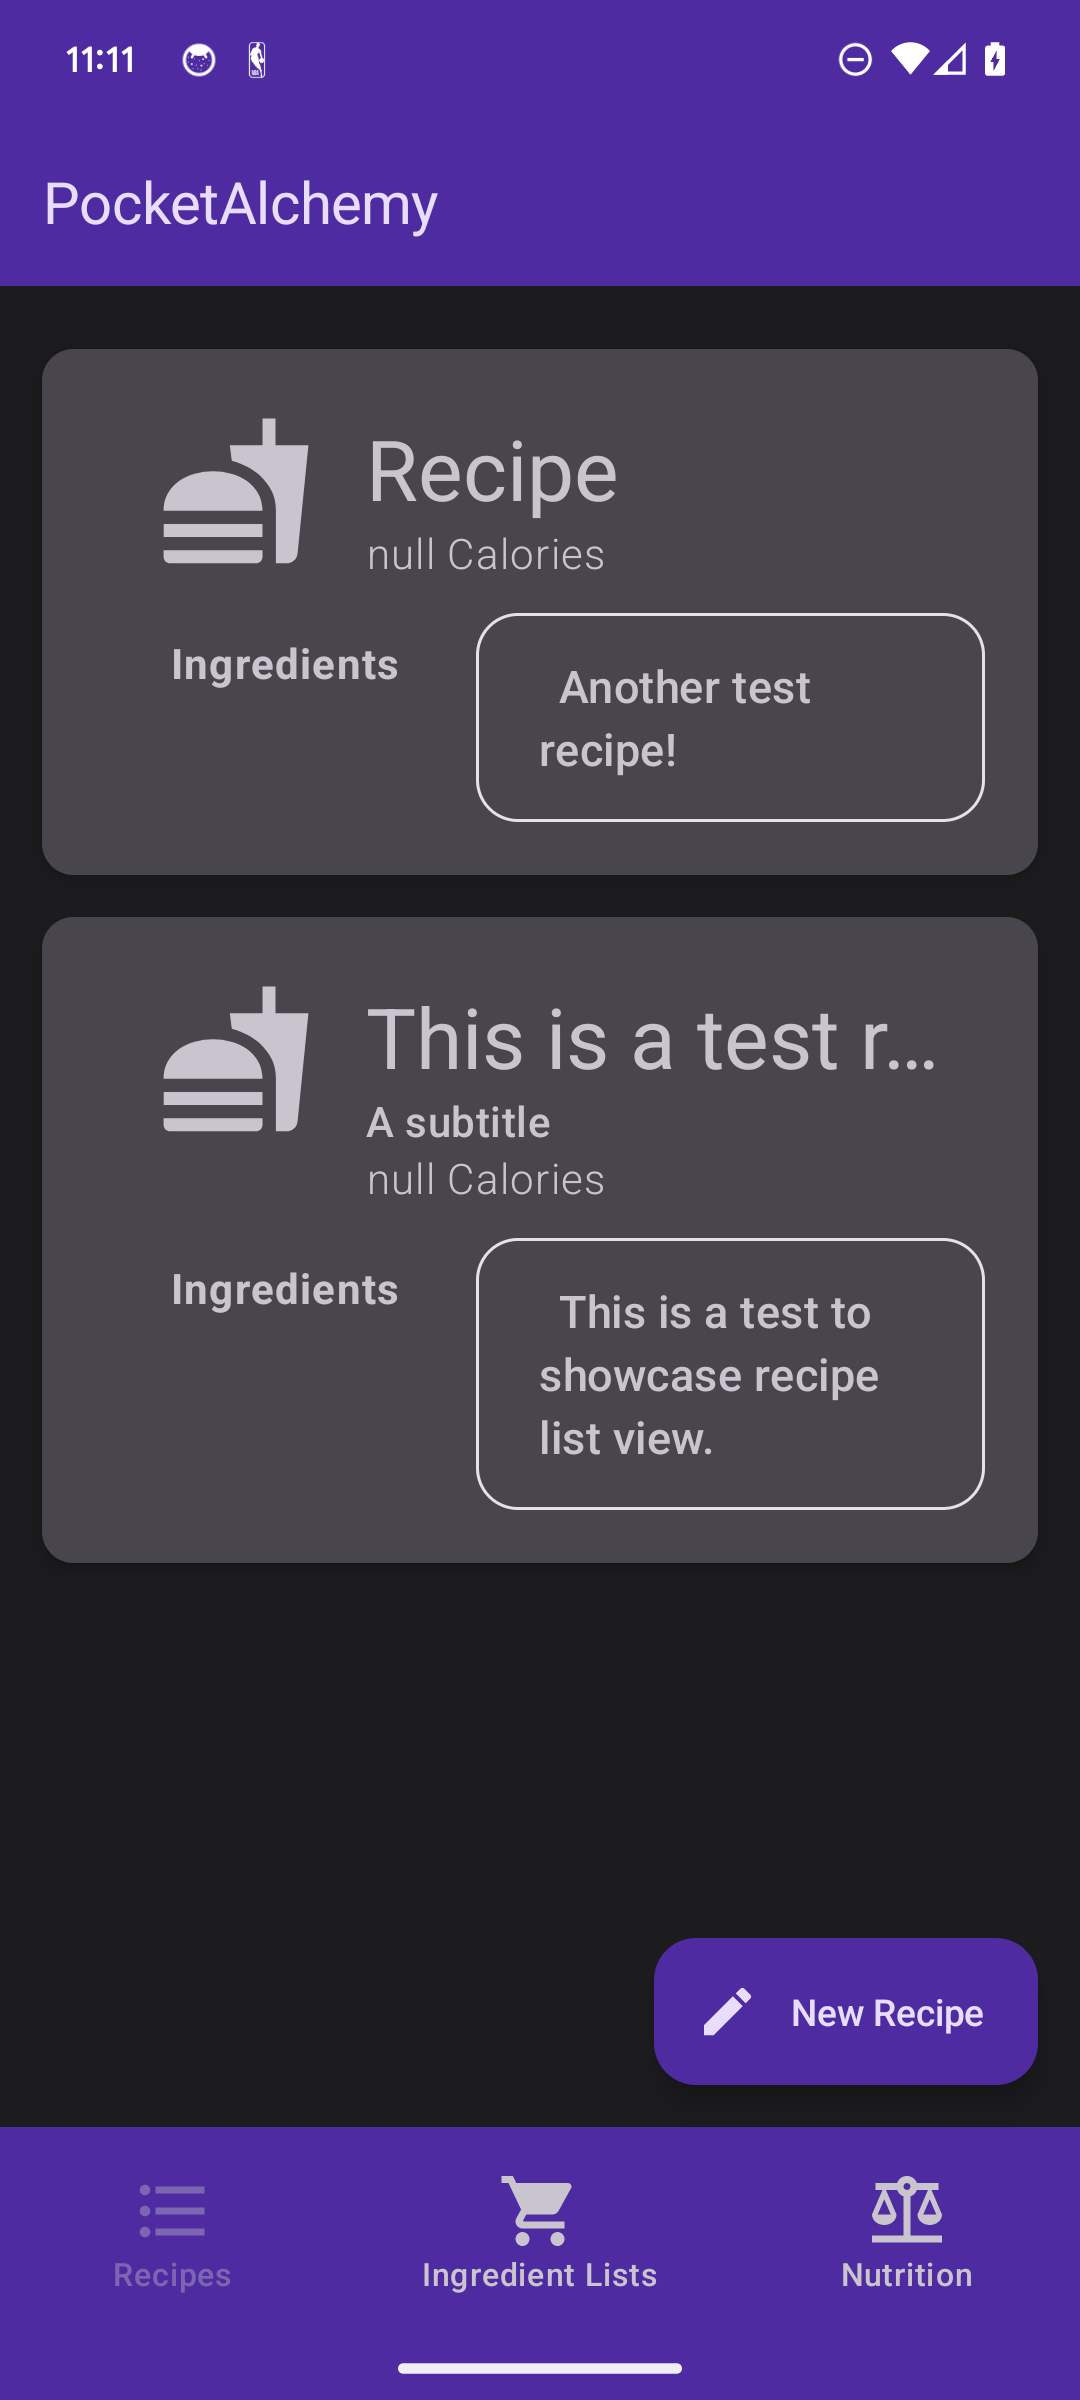
\includegraphics[scale=0.175]{../res/img/RecipeListDark.png}
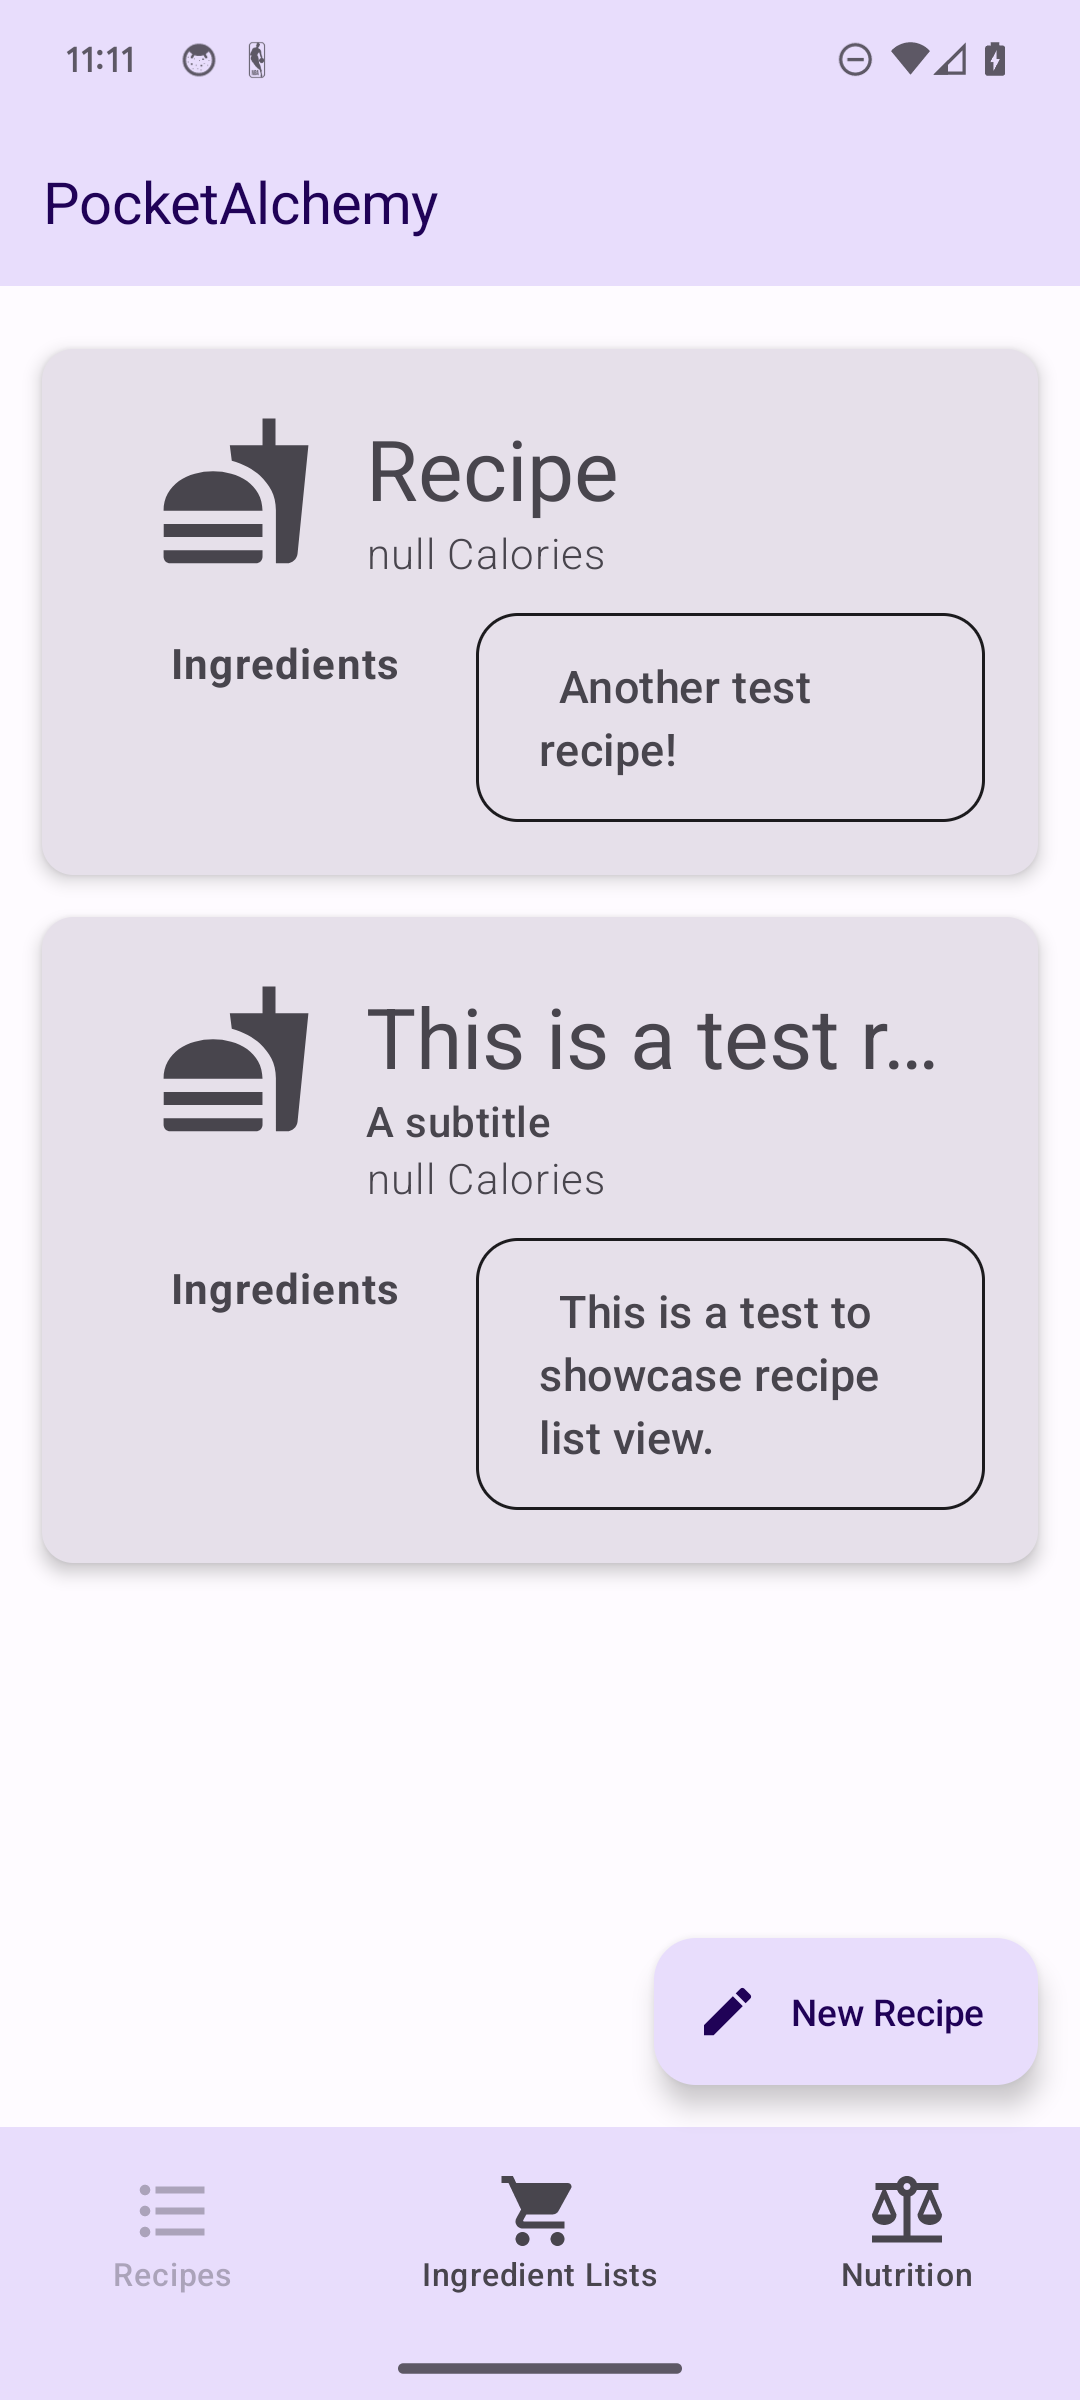
\includegraphics[scale=0.175]{../res/img/RecipeListLight.png}
\end{center}

\subsection{New Recipe}

\begin{center}
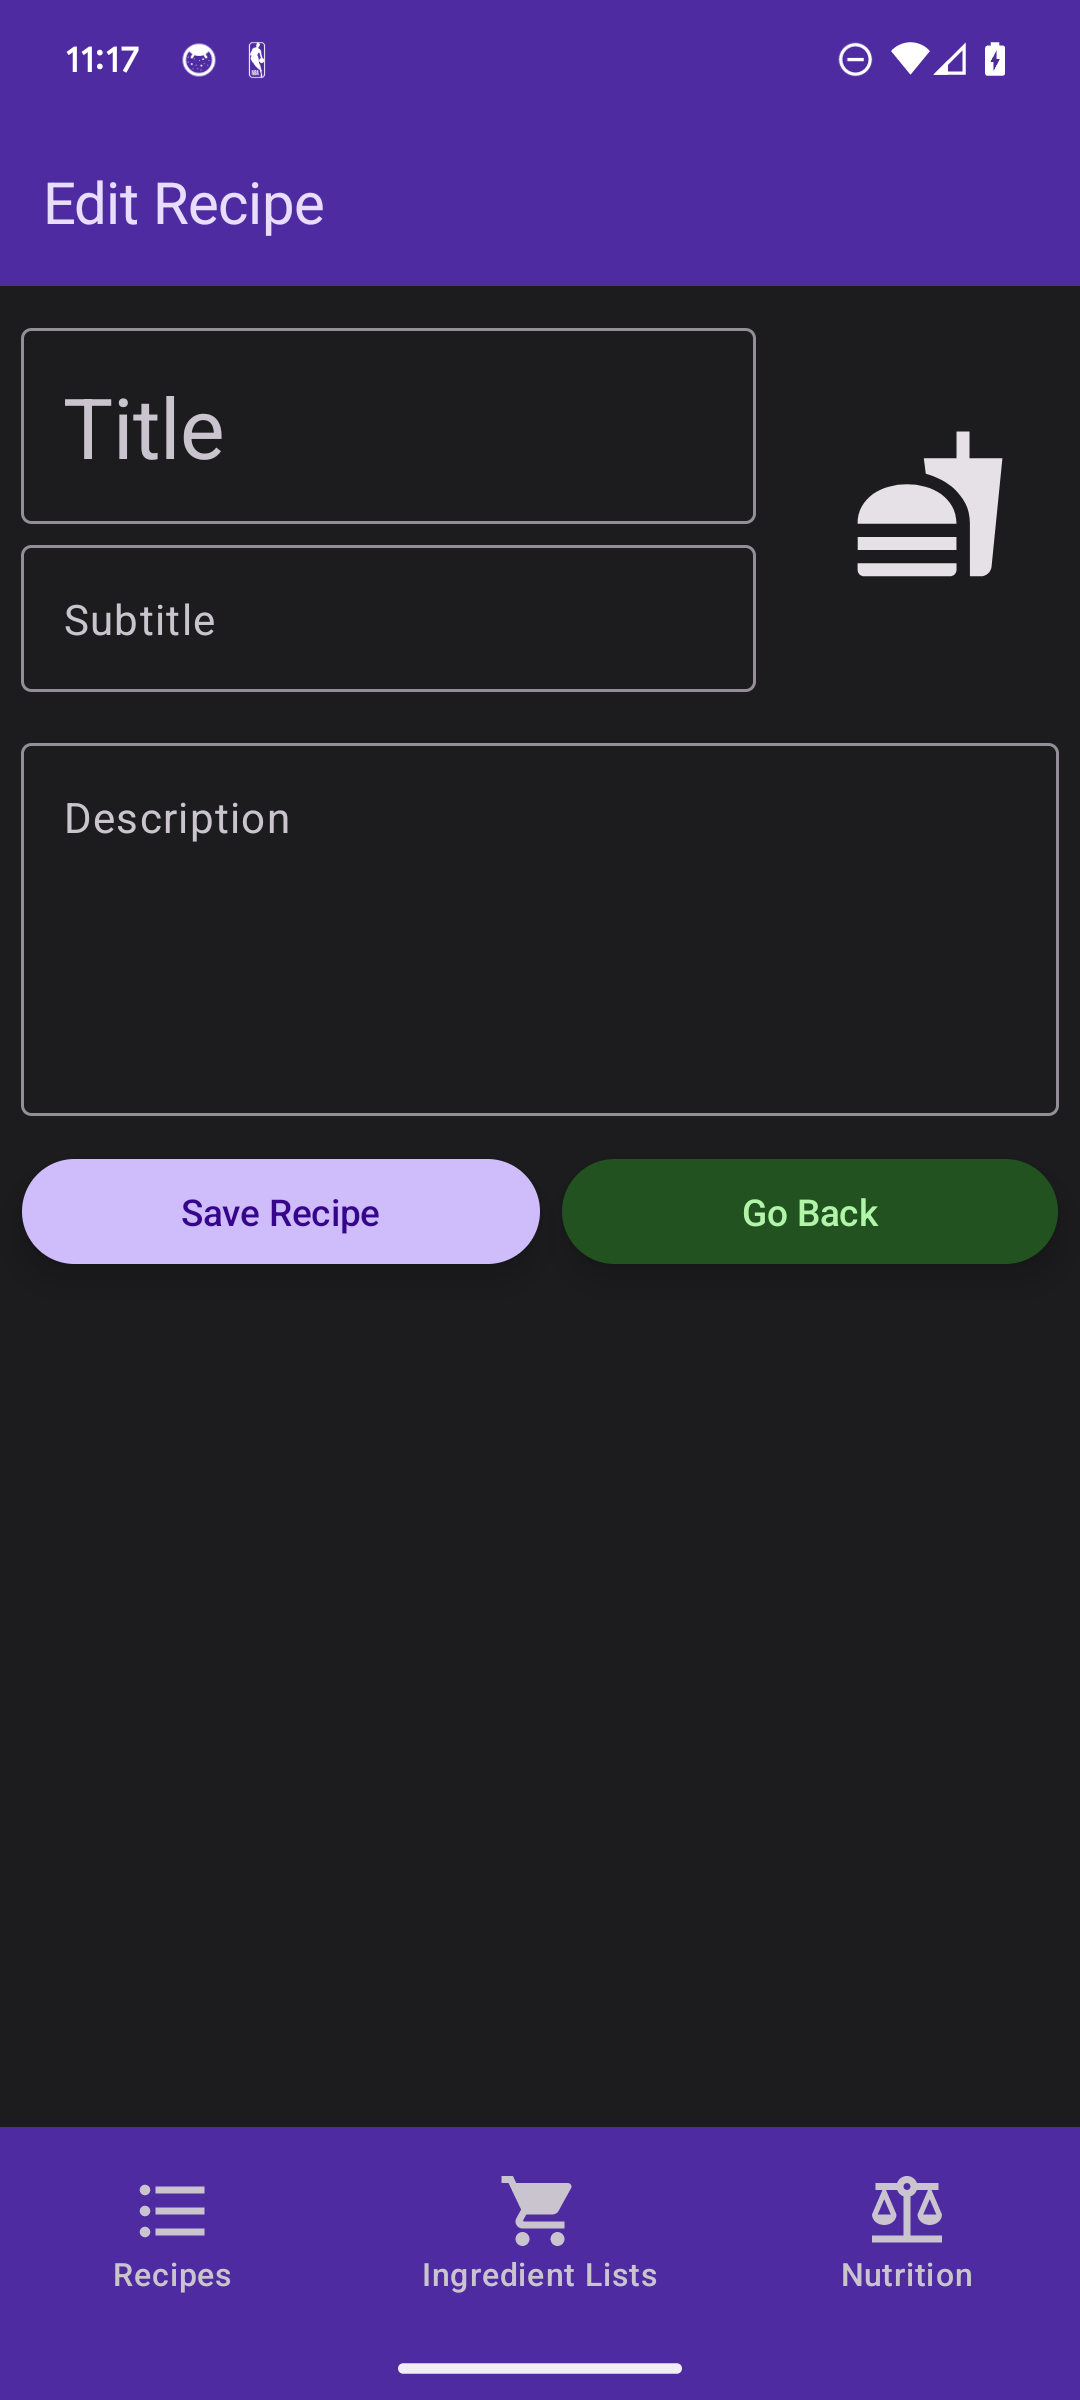
\includegraphics[scale=0.175]{../res/img/NewRecipeDark.png}
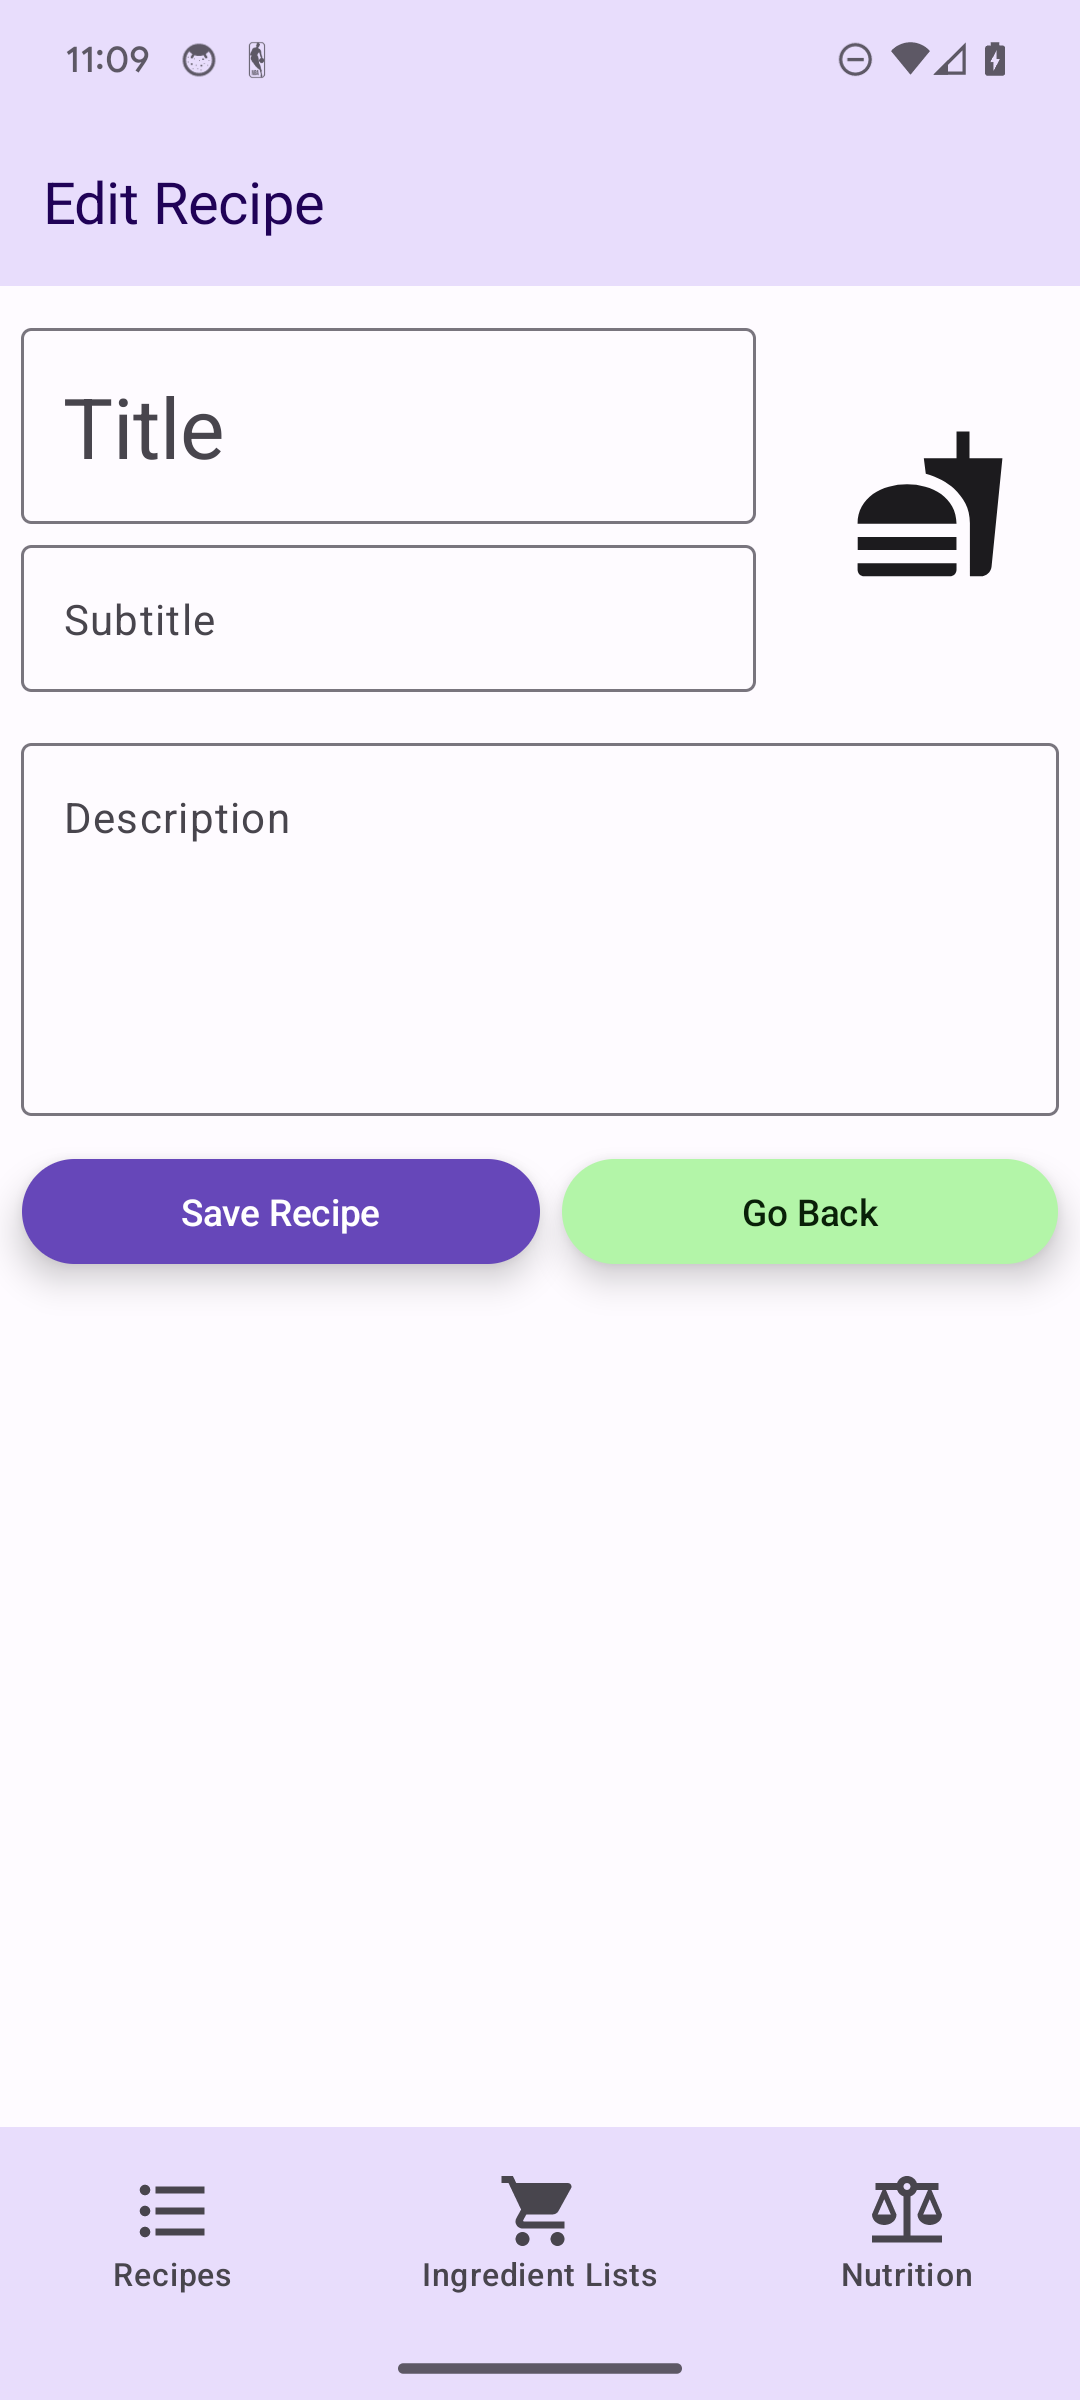
\includegraphics[scale=0.175]{../res/img/NewRecipeLight.png}
\end{center}

\subsection{Edit Recipe}

\begin{center}
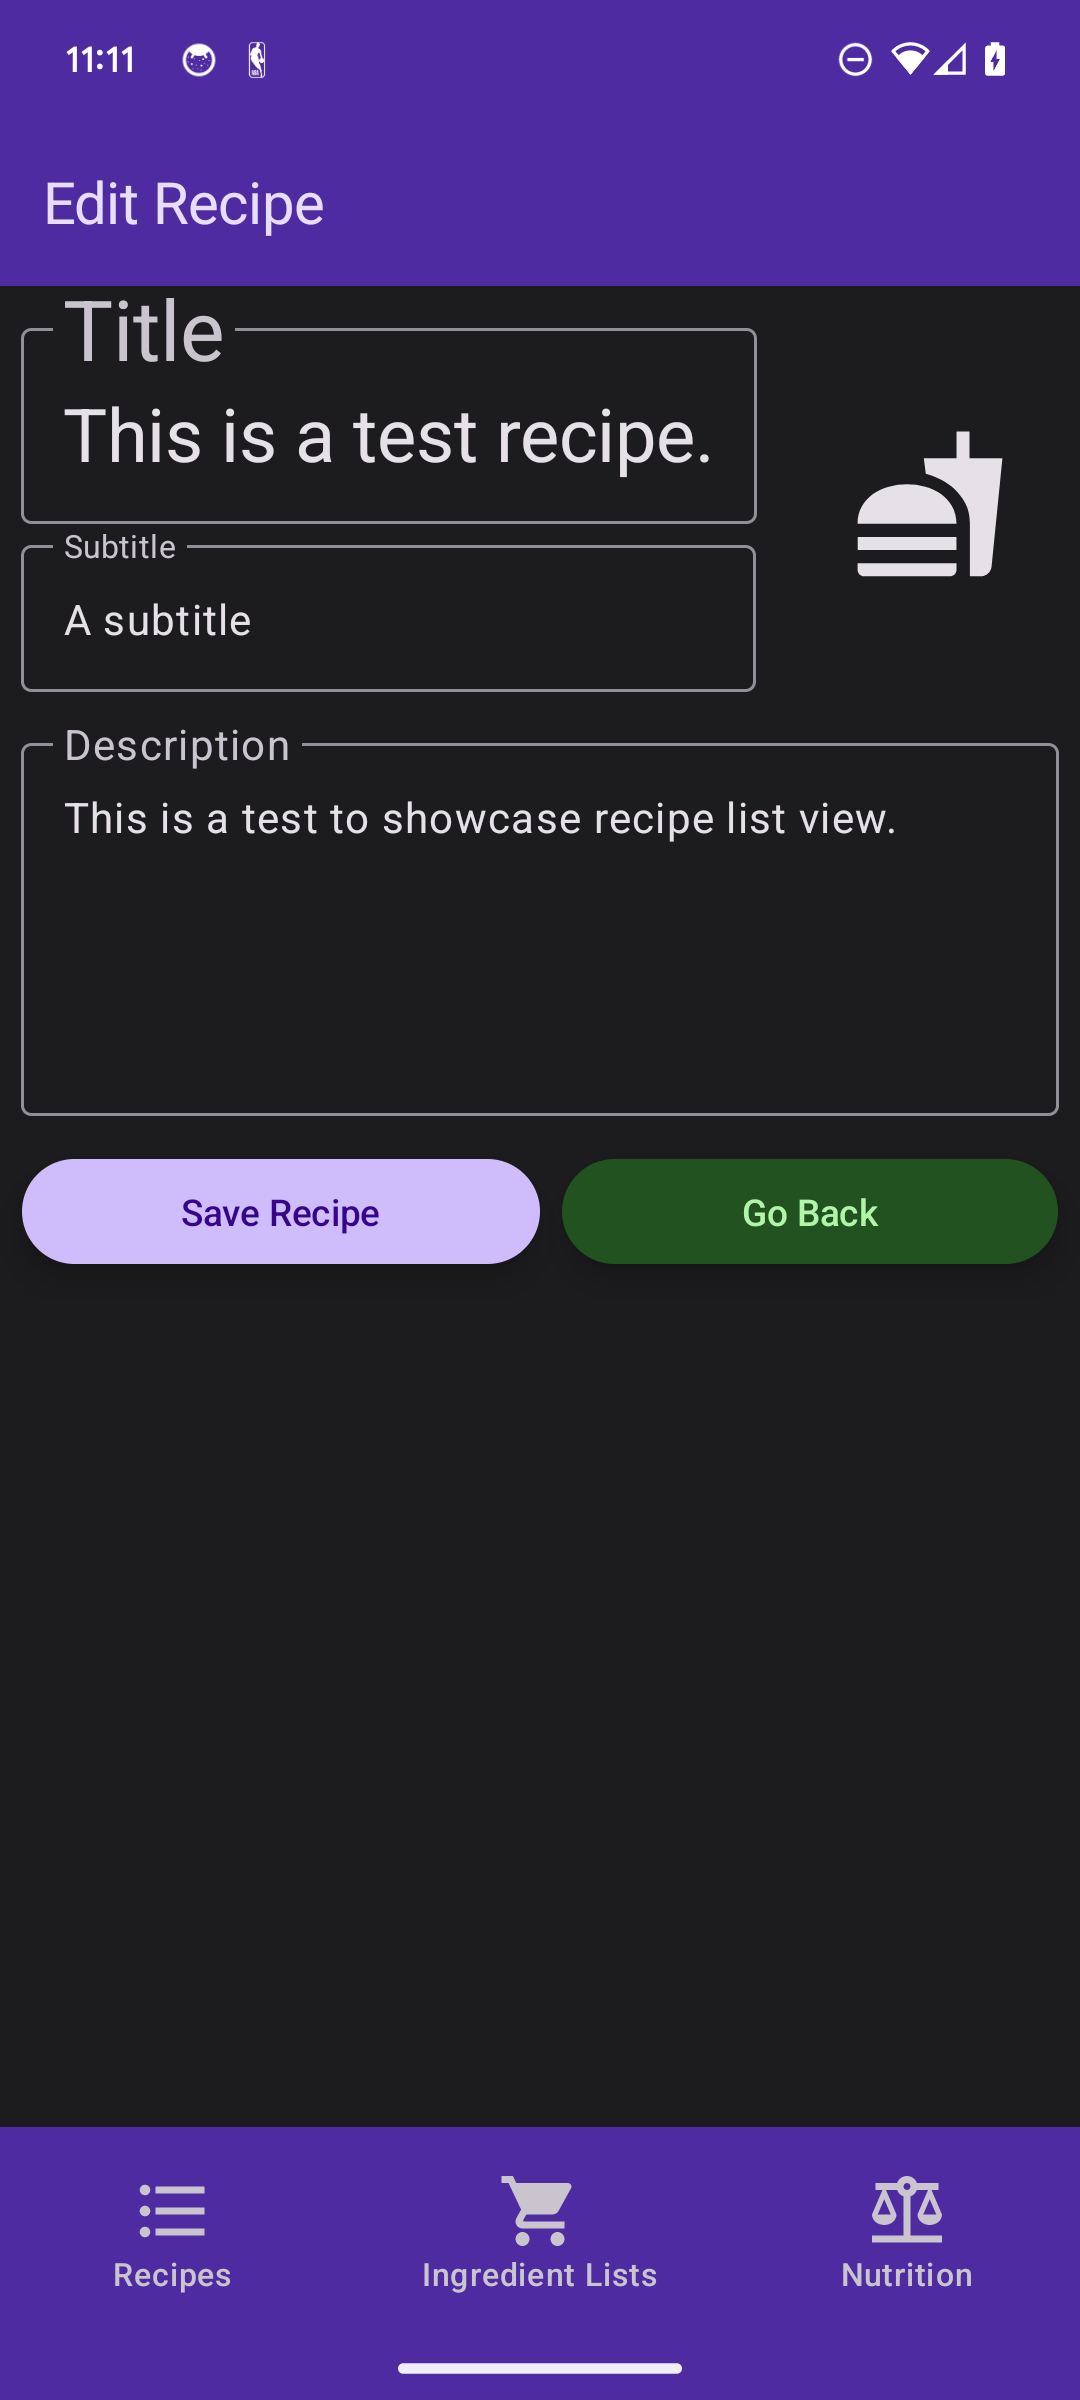
\includegraphics[scale=0.175]{../res/img/EditRecipeDark.png}
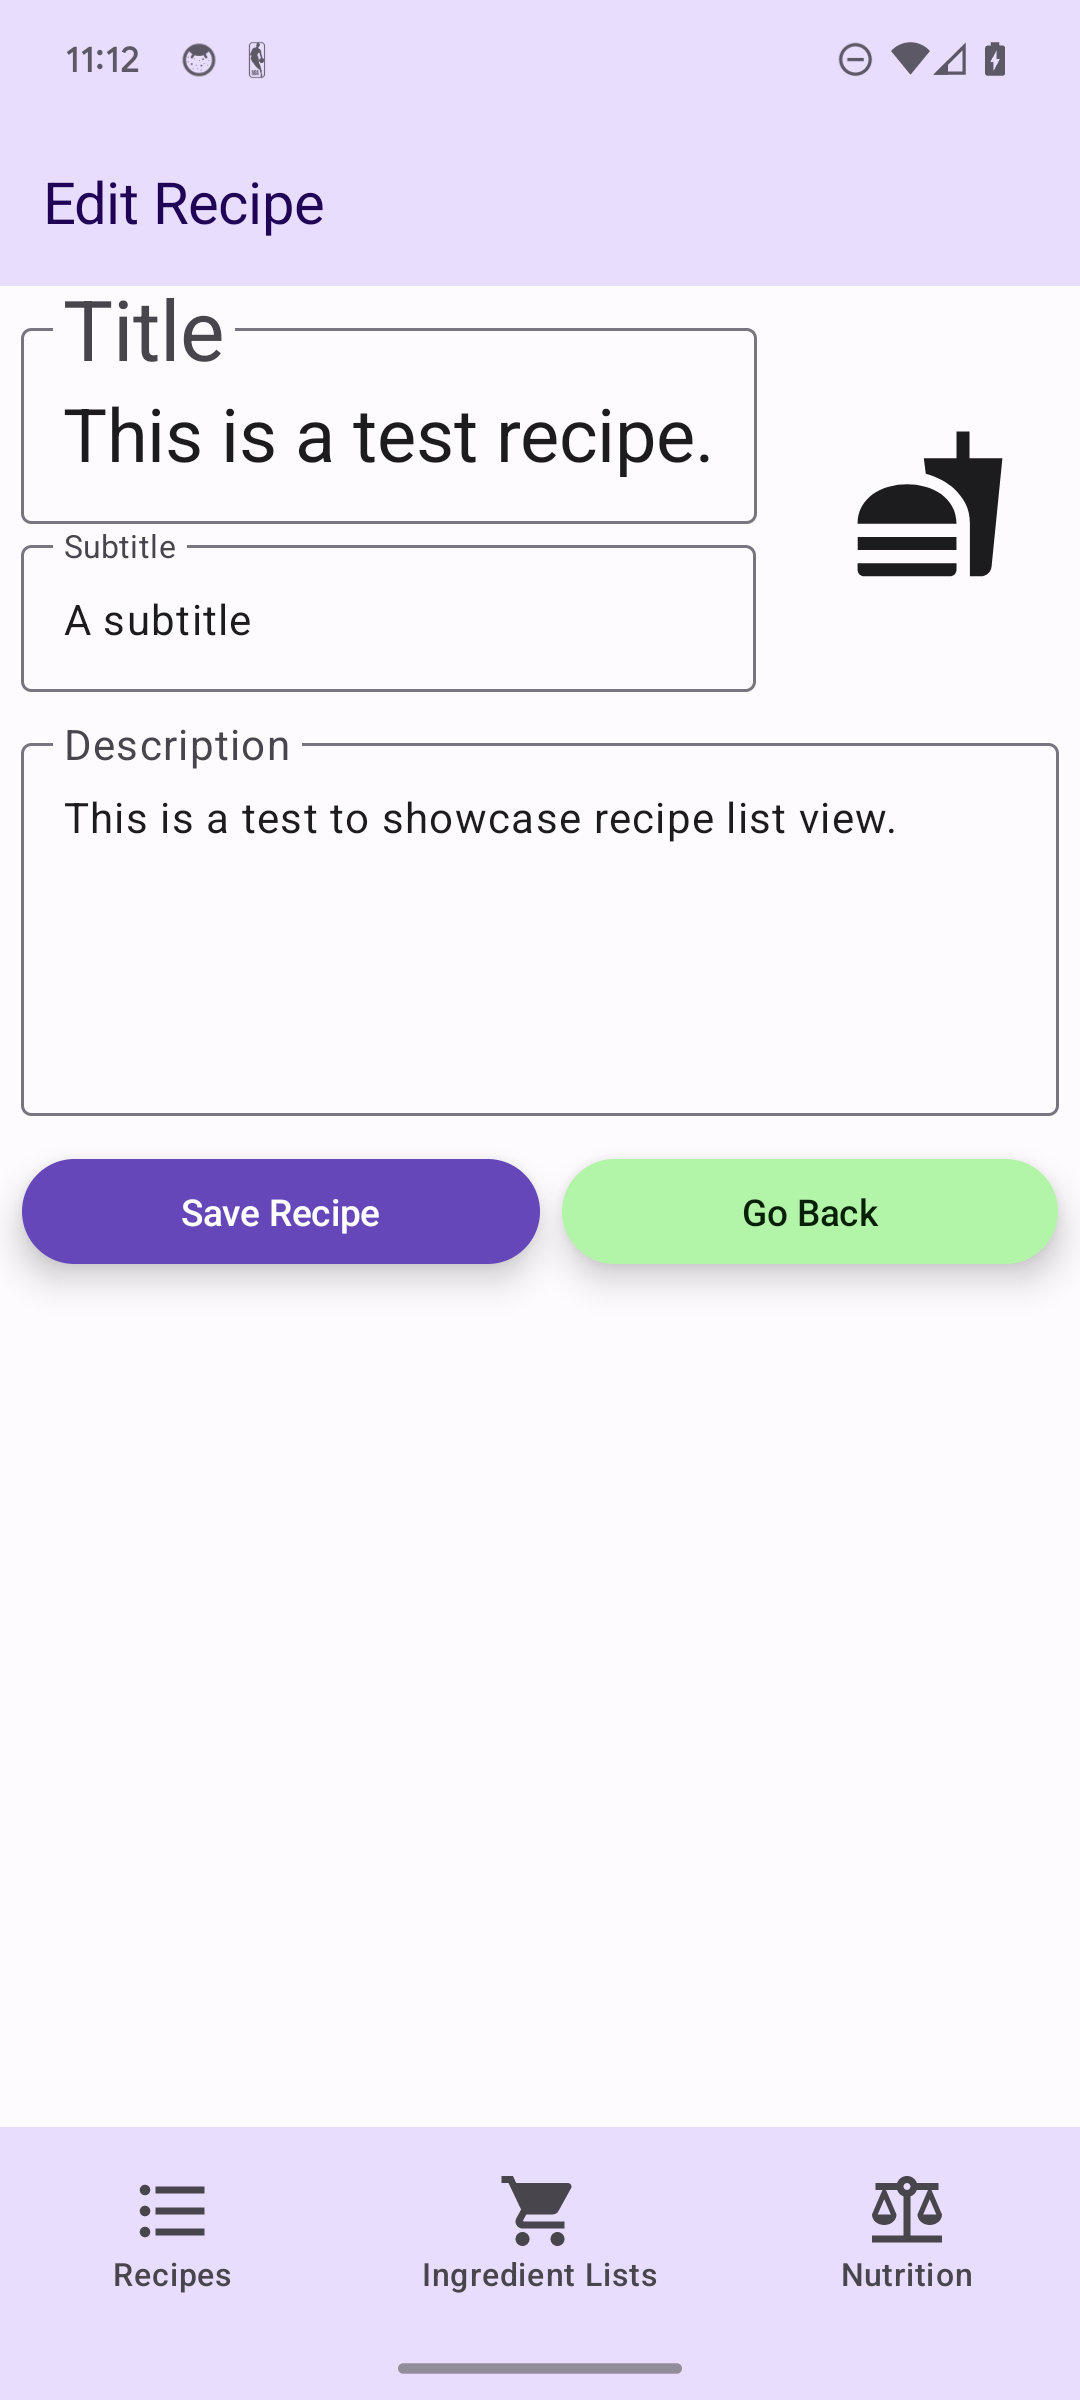
\includegraphics[scale=0.175]{../res/img/EditRecipeLight.png}
\end{center}
    
\end{document}